\chapter{Экспериментальная часть}

\section{Эксперименты}

\subsection{Корпус CoNLL 2003}

CoNLL 2003 \citep{tjong2003introduction} - англоязычный корпус для оценки качества
методов распознавания именованных сущностей.
Корпус содержит обучающую, тестовую и валидационную выборку.
Размечено 4 типа сущностей - персоны (PER), организации (ORG), локации (LOC) и другие (MISC).
Корпус размечен по схеме Inside, Outside, Begin (IOB).
Оценка качества считается с помощью F1-micro-average.

\begin{table}[ht]
  \caption{Количество статей, предложений, токенов и именованных сущностей}
  \centering
  \begin{tabular}{ | p{3cm} | p{1.5cm} | p{2.5cm} | p{1.5cm} | p{1cm} | p{1cm} | p{1cm}| p{1cm} |}
    \hline\hline
    Выборка & Статьи & Предложения & Токены & LOC & MISC & ORG & PER \\
    \hline
    Обучающая & 946 & 14987 & 203621 & 7140 & 3438 & 6321 & 6600 \\
    \hline
    Валидационная & 216 & 3466 & 51362 & 1837 & 922 & 1341 & 1842 \\
    \hline
    Тестовая & 231 & 3684 & 46435 & 1668 & 702 & 1661 & 1617 \\
    \hline
  \end{tabular}
\end{table}

Как и у \citep{collobert2011natural}, данные были сконвертированы из схемы IOB
в схему IOBES (Inside, Outside, Begin, End, Single).
Во время тестирования, данные конвертируются обратно в формат IOB и подаются на вход скрипта,
включенного в CoNLL 2003, оценивающего качество классификации.

\subsection{Синтактико-семантические признаки Compreno}
Синтактико-семантически признаки были получены с помощью Compreno.
Они представляют собой разреженные вектора размерности 83950.
Они покрывают около 60\% корпуса CoNLL 2003.
Все токены, не покрытые Compreno, кодировались как дополнительный признак 83951.

\subsection{Эксперименты без синтактико-семантических признаков}

Нейросетевая модель имеет такие же параметры как и у \citep{collobert2011natural}.
Небольшой модификацией является добавление Dropout слоя в качестве регуляризатора,
после каждого полносвязного слоя.
Размерность выходного слоя - 17. Четыре для каждого из четырех типов тегов и один для Outside.

В качестве векторного представления слов (embeddings в таблице \ref{table:raw_net}),
использовались Senna embeddings\footnote{http://ronan.collobert.com/senna/},
которые находятся в открытом доступе.

\begin{table}[ht]
  \caption{Результаты экспериментов без использования синтактико-семантических признаков}
  \centering
  \begin{tabulary}{\textwidth}{| L | L | L | L | L | L |}
    \hline\hline
    \multicolumn{1}{|p{1.5cm}|}{Модель} & Признаки & Выборка & Метод оптимизации & Полученная F1, \% & F1 в статье \cite{collobert2011natural} \\
    \hline
    Window & Embeddings, Capitalization & train & Mini-batch gradient descent & 86.27 & - \\
    \hline
    Window & Embeddings, Capitalization & train & Stochastic gradient descent & - & 86.97 \\
    \hline
    ConvNet + CRF & Embeddings, Capitalization, Position & train & Stochastic gradient descent & - & 88.67 \\
    \hline
    ConvNet + CRF & Embeddings, Capitalization, Position, Gazetteer & train & Stochastic gradient descent & - & 89.59 \\
    \hline
    ConvNet & Embeddings, Capitalization, Position & train & Stochastic gradient descent & 86.77 & - \\
    \hline
    ConvNet & Embeddings, Capitalization, Position, Gazetteer & train & Stochastic gradient descent & 87.89 & - \\
    \hline
    ConvNet & Embeddings, Capitalization, Position, Gazetteer & train + dev & Stochastic gradient descent & 88.37 & - \\
    \hline
    ConvNet & Embeddings, Capitalization, Position, Gazetteer & train & Mini-batch gradient descent & \textbf{87.49} & - \\
    \hline
  \end{tabulary}
  \label{table:raw_net}
\end{table}


По таблице \ref{table:raw_net} видно, что результаты немного ниже чем у \citep{collobert2011natural}.
Это связано с тем, что для Window подхода использован другой метод оптимизации,
а для Convolution подхода не были применены условные случайные поля.

В качестве референсной, будет использована модель из последнего эксперимента
показывающая 87.49\% F1.
Это сделано для чистоты эксперимента, т.к. далее  обучение происходило только
на обучающей выборке по правилам соревнования CoNLL 2003 и применялся mini-batch
gradient descent для ускорения экспериментов.

\subsection{Эксперименты с синтактико-семантическими признаками сжатыми с использованием SVD}

Синтактико-семантически признаки Compreno размерности 83950 были сжаты с использованием
TruncatedSVD\footnote{http://scikit-learn.org/stable/modules/generated/sklearn.decomposition.TruncatedSVD.html}
до размерности 1024.
После сжатия описываемая дисперсия была равна 72\%. Т.е. потерялось 28\% информации.
Сжатые вектора были добавлены в нейронную сеть с помощью дополнительного Lookup Table слоя.

\begin{table}[ht]
  \caption{Результаты с синтактико-семантическими признаками сжатыми SVD}
  \centering
  \begin{tabulary}{\textwidth}{| L | L | L | L | L | L |}
    \hline\hline
    \multicolumn{1}{|p{1.5cm}|}{Модель} & Признаки & Выборка & Метод оптимизации & Полученная F1, \% \\
    \hline
    ConvNet & Position, Compreno SVD 1024 & train & Mini-batch gradient descent & 75.89 \\
    \hline
    ConvNet & Capitalization, Position, Gazetteer, Compreno SVD 1024 & train & Mini-batch gradient descent & 81.83 \\
    \hline
    ConvNet & Embeddings, Capitalization, Position, Gazetteer, Compreno SVD 1024 & train & Mini-batch gradient descent & 86.85 \\
    \hline
    ConvNet & Embeddings, Capitalization, Position, Gazetteer & train & Mini-batch gradient descent & 87.49 \\
    \hline
  \end{tabulary}
  \label{table:svd_net}
\end{table}


По таблице \ref{table:svd_net} видно, что такой способ ведет к небольшому ухудшению F1-меры.


\subsection{Эксперименты с синтактико-семантическими признаками для совместно-оптимизированной нейросети}

Была добавлена еще одна нейронная сеть для синтактико-семантических признаков и оптимизирована
вместе со сверточной нейронной сетью.

Нейронная сеть для синтактико-семантических признаков работает следующим образом:
\begin{enumerate}
  \item На вход подается разреженный вектор признаков слова (размерность 83951) для которого предсказывается тег.
  \item Далее этот вектор пропускается через 2 полносвязных слоя.
  \item На выходе еще один полносвязный слой, который выдает вероятность определенного тега.
  Выходов также 17.
\end{enumerate}

Сверточная сеть, учитывающая всё предложение, и полносвязная сеть, обрабатывающая
синтактико-семантические признаки слова для которого предсказывается тег, соединяются следующим
образом (рис. \ref{figure:union_net}):
\begin{enumerate}
  \item Из обеих нейросетей удаляются выходные слои.
  \item Предыдущие слои из обеих сетей соединяются в новый полносвязный слой.
  \item Новый полносвязный слой соединяется с выходным слоем. Выходов как и тегов 17.
\end{enumerate}

\begin{figure}[h]
  \caption{Объединение двух нейросетей}
  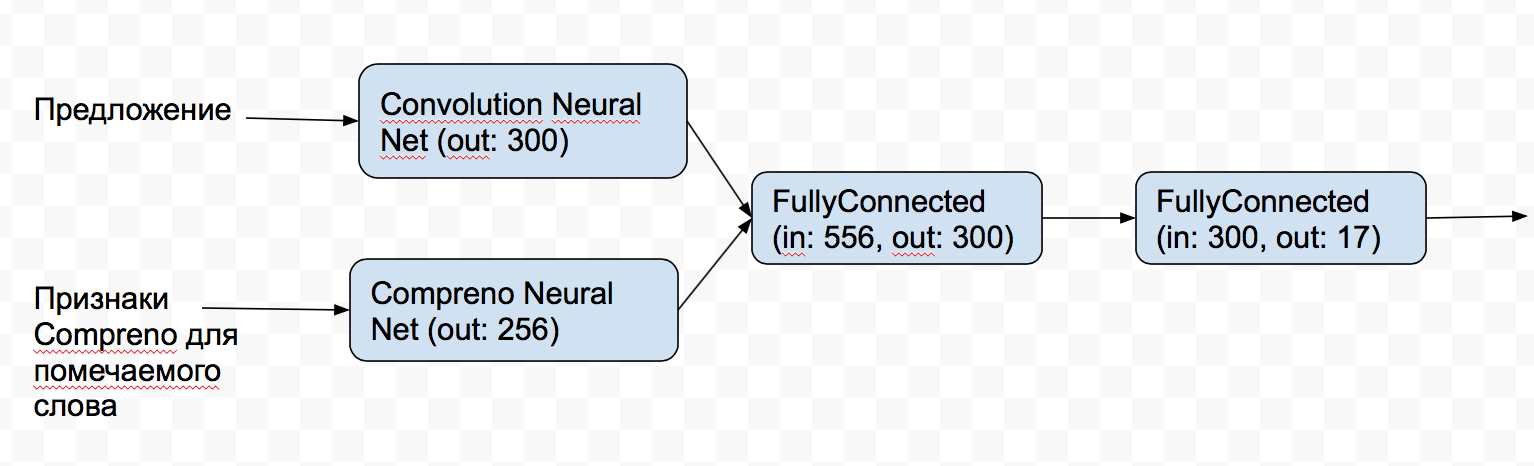
\includegraphics[scale=0.5]{two-net.png}
  \label{figure:union_net}
\end{figure}

Веса у объединенной сети были инициализированы обученными моделями -
моделью показывающую 87.49\% для сверточной сети и моделью показывающую
72.85\% (см. таблицу \ref{table:union_net}) для второй нейронной сети.

\begin{table}[ht]
  \caption{Результаты с синтактико-семантическими признаками для объединенной нейросети}
  \centering
  \begin{tabulary}{\textwidth}{| L | L | L | L | L | L |}
    \hline\hline
    \multicolumn{1}{|p{1.5cm}|}{Модель} & Признаки & Выборка & Метод оптимизации & Полученная F1, \% \\
    \hline
    Compreno Net & Compreno sparse features & train & Mini-batch gradient descent & 72.85 \\
    \hline
    ConvNet & Embeddings, Capitalization, Position, Gazetteer & train & Mini-batch gradient descent & 87.49 \\
    \hline
    ConvNet + Compreno Net & Embeddings, Capitalization, Position, Gazetteer, Compreno sparse features & train & Mini-batch gradient descent & \textbf{88.47} \\
    \hline
    ConvNet + Compreno Net & Embeddings, Capitalization, Position, Gazetteer, Compreno sparse features & train + dev & Mini-batch gradient descent & 88.81 \\
    \hline
  \end{tabulary}
  \label{table:union_net}
\end{table}

По таблице \ref{table:union_net} видно, что признаки Compreno улучшают F1-меру почти на один процент.
